Система контроля версий (СКВ) — это система, регистрирующая изменения в одном или нескольких файлах с тем, чтобы в дальнейшем была возможность вернуться к определённым старым версиям этих файлов.

Для разработки программного комплекса решено использовать Git.

Git  — распределённая система управления версиями файлов. Проект был создан Линусом Торвальдсом для управления разработкой ядра Linux, как противоположность системе управления версиями Subversion (также известная как «SVN») \cite{progit}.

Преимущества использования системы версий, очевидны:
\begin{itemize}
\item возможность возвращать к прежнему состоянию отдельные файлы или весь проект;
%\item возможность создавать свои ветки, не мешая при этом другим разработчикам;
\item возможность удалённой работы с текстами программ;
\item доступ к последним изменениям в коде, т.к. всё хранятся на сервере github.com;
\item тексты программ открыты, доступ к ним можно получить доступ в интернет;
%\item удобство работы с tex документами;
\item просматривать происходящие со временем изменения.
\end{itemize}

Основные постулаты работы в системе Git:
\begin{itemize}
\item каждая задача решается в своей ветке;
\item сохраняем изменения сразу, как что-то получили осмысленное;
%\item в master мержится не разработчиком, а вторым человеком, который производит вычитку и тестирование изменения;
\item все сохранённые изменения должны быть осмысленно подписаны/прокомментированы.
\end{itemize}
\begin{figure}[ht]
\center{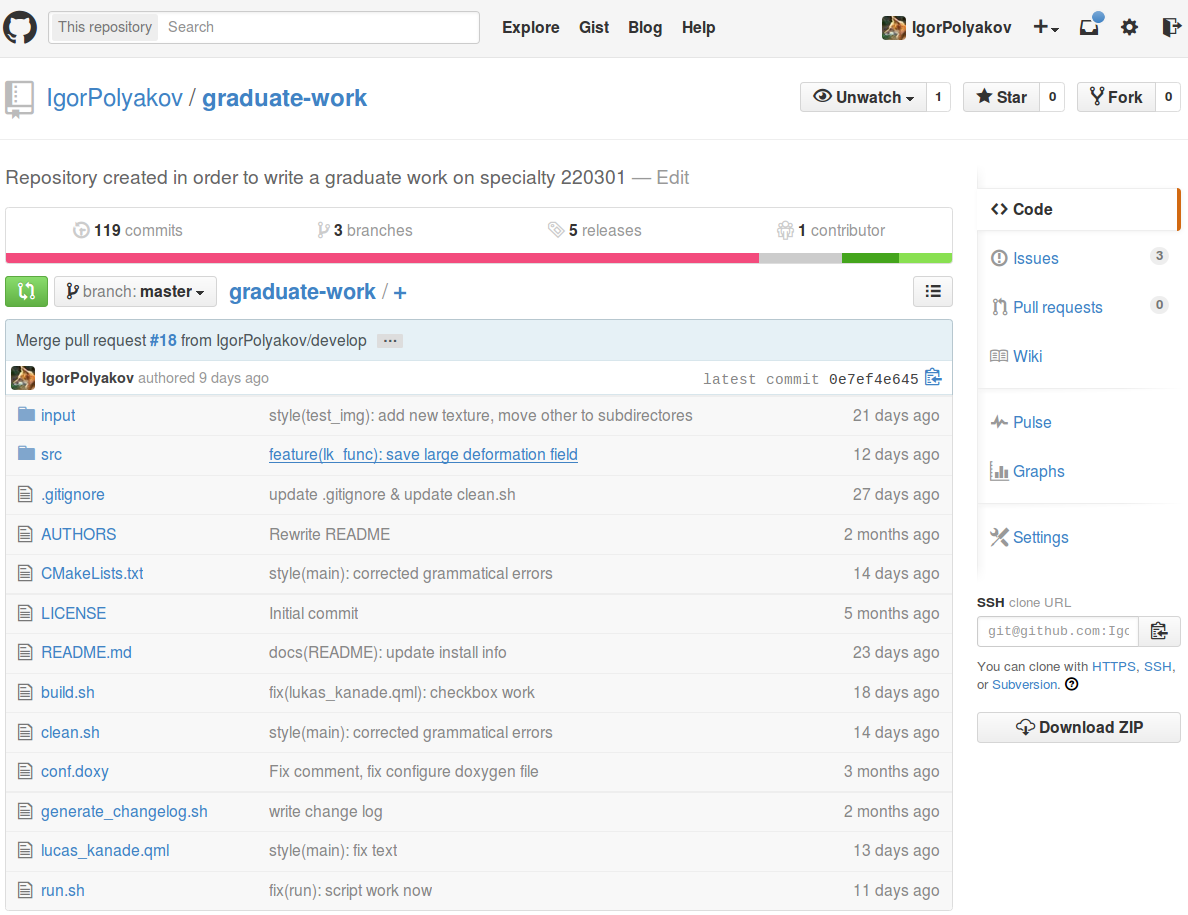
\includegraphics[width=0.9\linewidth]{github}}
\caption{Тексты программ в репозитории github}
\label{pic:github}
\end{figure}

Для работы над проектом был использован репозиторий на сервере github.com. Слепок последних изменений из репозитория можно взять по адресу: git clone git@github.com:IgorPolyakov/graduate-work.git

